%=============================================================================
% CHAPTER 3: METHODOLOGY
%=============================================================================
\chapter{Methodology}

\section{Overview}

In this chapter, I describe the methodology I followed to transform the theoretical background into a practical, functional password strength evaluation tool. My approach was iterative: I started by analysing requirements, then designed a modular architecture, implemented the core logic in Python, and systematically improved the tool through 18 enhancements and a user-experience redesign. Throughout this process, I focused on modularity, usability, and user privacy.

The iterative development process followed this general pattern: (1) define requirements and design the architecture, (2) implement the initial version of each module, (3) test the tool with representative passwords and identify weaknesses, (4) implement targeted improvements, and (5) repeat from step 3 until the tool met the desired quality standards. This process resulted in 18 documented enhancements covering scoring accuracy, pattern detection coverage, dictionary comparison, user interface improvements, and overall code quality. A subsequent user-experience redesign restructured the interface from a basic layout to a two-column analysis dashboard with animated visual indicators.

\clearpage

\section{System Requirements and Technology Justification}

The tool was developed to run as a desktop application on the Windows operating system. The technical requirements are as follows:

\begin{itemize}
    \item \textbf{Programming language:} Python 3.14, selected for its readability, strong string manipulation capabilities, extensive standard library, and support for modern type annotations.
    \item \textbf{GUI framework:} CustomTkinter (version 5.2.0 or later), a modern wrapper around Tkinter that provides native-looking dark-themed widgets with minimal configuration.
    \item \textbf{Platform:} Windows desktop. The application creates a fixed-size, non-resizable window (1000$\times$780 pixels) centred on the screen.
    \item \textbf{Network:} No network connection is required. All processing happens locally, and no passwords are stored, logged, or transmitted at any point.
    \item \textbf{Hardware assumptions for crack time estimation:} The tool assumes an attacker capable of 10 billion guesses per second, consistent with modern GPU-based cracking rigs.
\end{itemize}

The only external dependency beyond the Python standard library is CustomTkinter. All other modules---\texttt{math}, \texttt{re}, \texttt{secrets}, \texttt{string}, \texttt{os}, \texttt{sys}, \texttt{dataclasses}---are part of the Python standard library, minimising installation complexity and reducing the attack surface of the application.

\subsection{Why Python}

Python was chosen as the programming language for this project for several compelling reasons:

\begin{itemize}
    \item \textbf{Readability and maintainability:} Python's syntax emphasises clarity and uses indentation to define code blocks, resulting in code that is easy to read, review, and maintain. For a thesis project that must be understood and evaluated by others, this readability is a significant advantage over more verbose languages such as Java or C++.

    \item \textbf{Rapid development:} Python's dynamic typing, interactive interpreter, and concise syntax allow features to be prototyped and tested quickly. This was particularly valuable during the iterative development process, where 18 enhancements and a UX redesign were implemented in rapid succession.

    \item \textbf{Strong standard library:} Python's standard library provides built-in modules for regular expressions (\texttt{re}), mathematical operations (\texttt{math}), cryptographic random number generation (\texttt{secrets}), string manipulation (\texttt{string}), and immutable data structures (\texttt{dataclasses}). These modules eliminated the need for external dependencies for all core evaluation logic.

    \item \textbf{String manipulation ergonomics:} Password evaluation is fundamentally a string-analysis task. Python's first-class Unicode support, slicing syntax, list comprehensions, and generator expressions make string processing operations concise and expressive. A pattern detection function that requires 20 lines in Python might require 40--60 lines in Java or C++ due to the absence of these conveniences.

    \item \textbf{Type annotations:} Python 3.14 supports modern type annotations (e.g., \texttt{list[str]}, \texttt{dict[str, bool]}, \texttt{str | None}), which improve code documentation and enable static type checking with tools like \texttt{mypy}. The \texttt{EvaluationResult} dataclass uses typed fields, making the API contract explicit and self-documenting.

    \item \textbf{Portability and cross-platform capability:} While the current implementation targets Windows, Python runs on all major operating systems. The evaluation engine (evaluator, entropy, patterns, dictionary\_check) has no platform-specific code and could be used on Linux or macOS without modification. Only the GUI module would need minor adjustments for platform-specific font rendering.
\end{itemize}

\textbf{Why not alternative languages?} Java was considered but rejected due to its verbosity (boilerplate class definitions, explicit type declarations, and getter/setter patterns) and its lack of concise string processing syntax. C++ was rejected because manual memory management and pointer arithmetic add unnecessary complexity for a string-processing application with no performance-critical bottlenecks. JavaScript was rejected because browser-based tools raise privacy concerns---the password must be processed client-side with no server transmission, which is harder to guarantee in a web environment where network requests can be made invisibly. Python's local-only execution model provides a stronger guarantee of privacy by default.

\subsection{Library-by-Library Justification}

Each module and library used in the project was selected for a specific reason:

\begin{itemize}
    \item \textbf{\texttt{re} (regular expressions):} Used for character classification in the entropy module. Pre-compiled regex patterns (\texttt{\_RE\_LOWER}, \texttt{\_RE\_UPPER}, \texttt{\_RE\_DIGIT}, \texttt{\_RE\_SPECIAL}) efficiently determine which character categories appear in the password. Pre-compilation avoids the overhead of recompiling the same patterns on every call, which is important because \texttt{classify\_characters()} may be called multiple times per evaluation (once for entropy and once for diversity scoring).

    \item \textbf{\texttt{math} (mathematical functions):} Used for the $\log_2$ computation in the entropy formula $H = L \times \log_2 N$. Python's \texttt{math.log2()} function provides high-precision floating-point results, which is essential for accurate entropy estimation and crack time calculation.

    \item \textbf{\texttt{secrets} (cryptographic random number generation):} Used exclusively for password generation. The \texttt{secrets} module draws from the operating system's cryptographically secure random number generator (e.g., \texttt{CryptGenRandom} on Windows, \texttt{/dev/urandom} on Linux), unlike the \texttt{random} module's Mersenne Twister algorithm, which is statistically adequate but not cryptographically secure. The decision to use \texttt{secrets.choice()} for character selection and \texttt{secrets.SystemRandom().shuffle()} for randomisation ensures that generated passwords cannot be predicted even if an attacker knows the internal state of the random number generator.

    \item \textbf{\texttt{dataclasses} (structured data):} Used to define the \texttt{EvaluationResult} dataclass with \texttt{frozen=True}, which creates an immutable, typed, and self-documenting result object. The immutability guarantee prevents accidental modification of results after creation, and the automatic generation of \texttt{\_\_init\_\_}, \texttt{\_\_repr\_\_}, and \texttt{\_\_eq\_\_} methods reduces boilerplate code. The dataclass also includes per-dimension score breakdown fields (\texttt{length\_pts}, \texttt{diversity\_pts}, \texttt{entropy\_pts}, \texttt{pattern\_pts}, \texttt{dict\_pts}), enabling the GUI to display a detailed breakdown of how each dimension contributed to the final score.

    \item \textbf{\texttt{frozenset} (immutable set for O(1) membership testing):} Used in the pattern detection module to define \texttt{\_ASCII\_LOWER}, \texttt{\_ASCII\_UPPER}, and \texttt{\_ASCII\_DIGIT} as immutable sets. The use of \texttt{frozenset} rather than \texttt{set} makes the intent clear (these collections never change) and provides $O(1)$ average-case membership testing for the character filtering step in \texttt{detect\_sequential()}, which is called on every evaluation.

    \item \textbf{CustomTkinter (GUI framework):} Selected over several alternatives for the graphical interface:
    \begin{itemize}
        \item \textbf{Over plain \texttt{tkinter}:} Standard Tkinter provides basic widgets but lacks modern styling (dark themes, rounded corners, smooth animations). CustomTkinter wraps Tkinter with a modern aesthetic while retaining its simplicity and cross-platform compatibility.
        \item \textbf{Over PyQt / PySide:} The Qt framework is powerful but introduces a large external dependency (30+ MB), a complex licensing model (GPL vs.\ LGPL vs.\ commercial), and a steeper learning curve. For a focused thesis project, the additional capability is unnecessary.
        \item \textbf{Over Kivy:} Kivy targets mobile and touch interfaces, which is not the deployment target. Its custom rendering engine also produces a non-native look and feel on desktop platforms.
    \end{itemize}
    CustomTkinter provides the ideal balance: a single lightweight dependency, native-looking dark-themed widgets, and full access to the underlying Tkinter canvas for custom drawing (the semicircular gauge).
\end{itemize}


\section{Architecture}

The tool is structured as a Python package called \texttt{password\_tool} containing five core modules, each with a distinct responsibility. This modular design ensures separation of concerns: the evaluation logic is entirely independent of the graphical interface and can be tested and used in isolation.

\begin{itemize}
    \item \textbf{main.py} --- Graphical user interface. Defines the \texttt{PasswordAnalyzerApp} class, which creates the CustomTkinter window, handles user input, and displays evaluation results. This module is the only one that depends on CustomTkinter.
    \item \textbf{evaluator.py} --- Scoring engine. Combines the five analysis dimensions into a single 0--100 score and returns an immutable \texttt{EvaluationResult} dataclass. Also contains the \texttt{generate\_password} function.
    \item \textbf{entropy.py} --- Entropy calculation. Implements Shannon entropy estimation, character classification, entropy-to-score mapping, and brute-force crack time estimation.
    \item \textbf{patterns.py} --- Pattern detection. Detects sequential characters, repeated characters, and keyboard-row patterns (including reversed variants).
    \item \textbf{dictionary\_check.py} --- Dictionary comparison. Provides exact match, substring detection, and Levenshtein distance similarity checking against a common-passwords list.
\end{itemize}

Supporting files include \texttt{\_\_init\_\_.py} (marks the directory as a Python package), \texttt{\_\_main\_\_.py} (entry point for \texttt{python -m password\_tool}), and \texttt{common\_passwords.txt} (a curated list of 181 common and leaked passwords). The external files \texttt{requirements.txt} and \texttt{run.bat} manage dependencies and provide a convenient Windows launcher.

\begin{figure}[H]
    \centering
    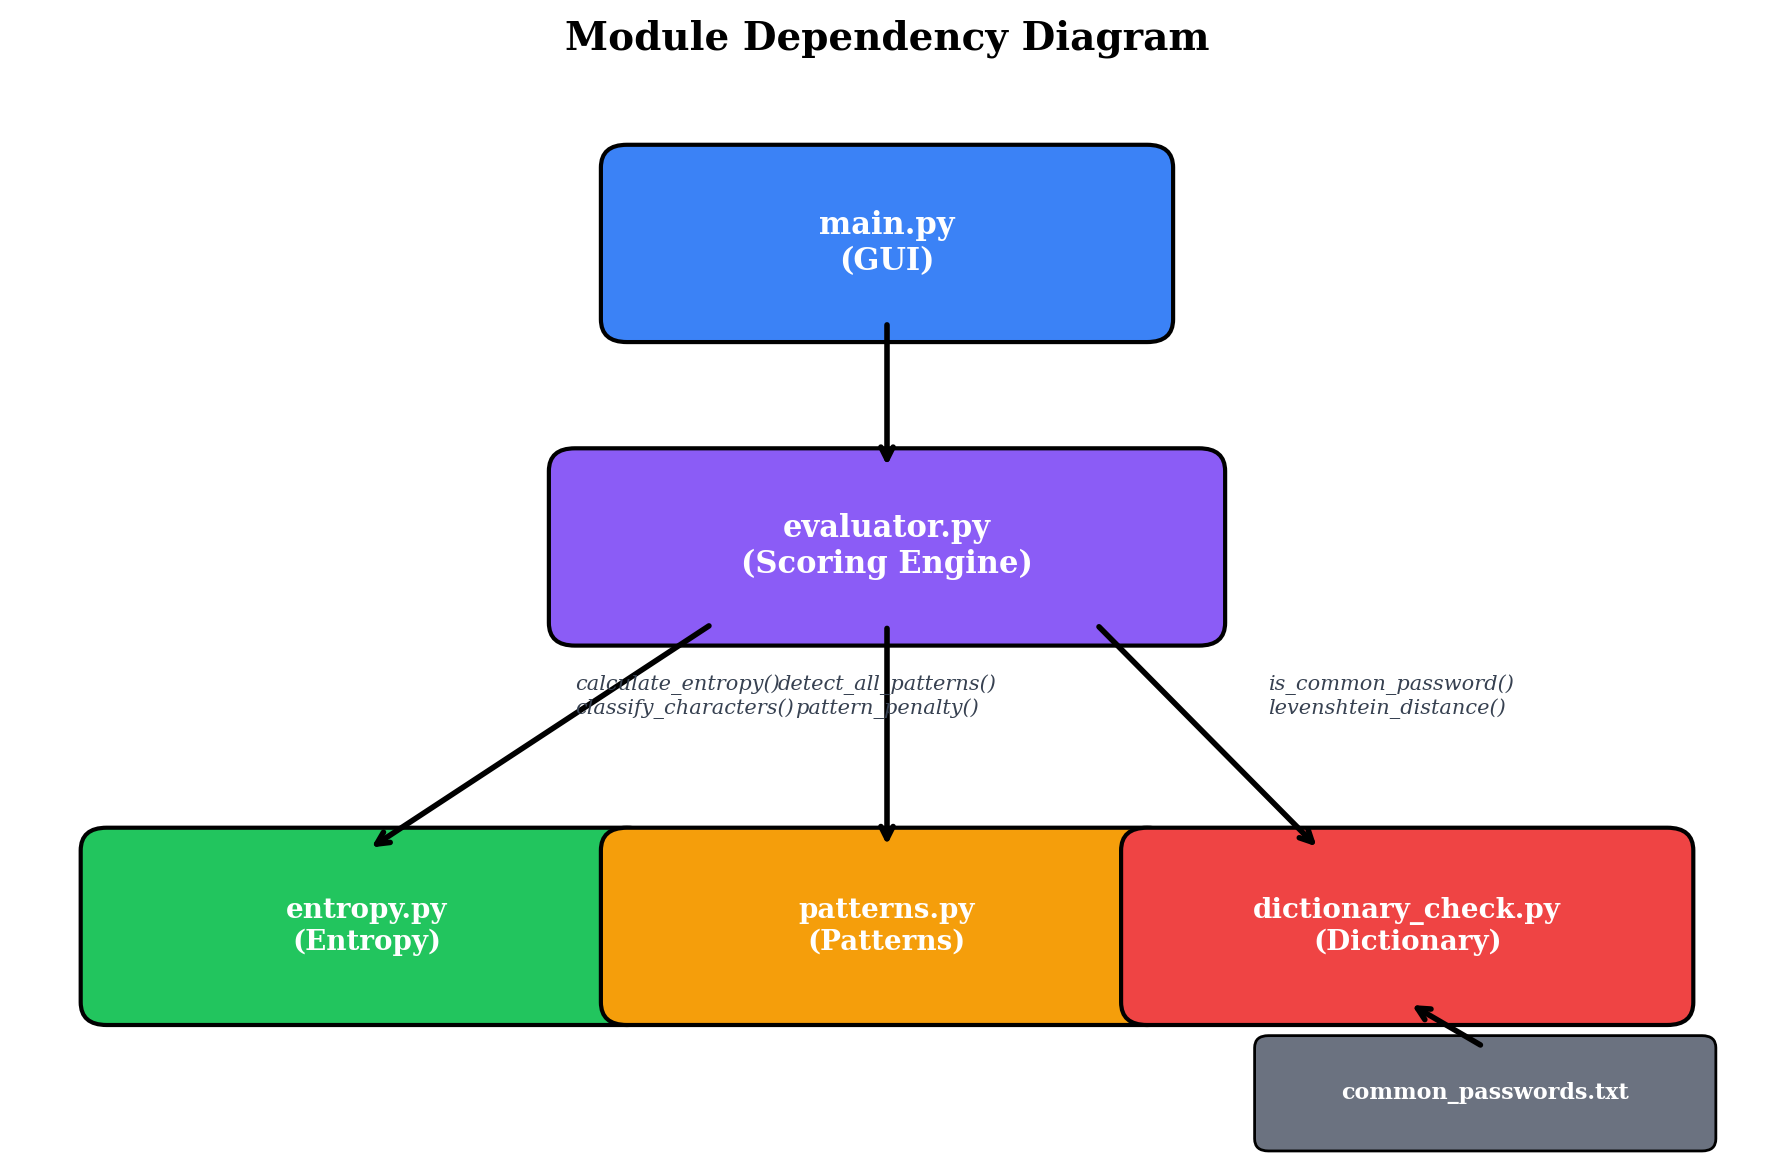
\includegraphics[width=0.85\textwidth]{figures/module_dependency_flowchart.png}
    \caption{Module dependency diagram illustrating the flow of data between components.}
    \label{fig:module_flow}
\end{figure}

The key design principle is that \texttt{evaluator.py} serves as the single orchestrator: it calls the three analysis modules, combines their results, and produces the final evaluation. The GUI module (\texttt{main.py}) only communicates with the evaluator and never directly accesses the analysis modules. This ensures that the evaluation logic remains consistent regardless of how it is invoked, and that the analysis modules can be modified or extended without affecting the GUI.


\section{Evaluation Algorithm}

The core of the tool is a five-dimension hybrid scoring model that produces a single integer score from 0 to 100. Each dimension contributes a specific portion of the final score, and the combination of positive scores and negative penalties ensures that both strengths and weaknesses are reflected in the result.

\subsection{Scoring Dimensions}

The five scoring dimensions are:

\begin{enumerate}
    \item \textbf{Length score (0--25):} Rewards longer passwords with progressively higher scores. Passwords of 16 or more characters receive the maximum of 25 points, while passwords shorter than 6 characters receive 0.

    \item \textbf{Character diversity score (0--25):} Evaluates how many of the four character categories (lowercase, uppercase, digits, special characters) are present. Each category contributes 6 points, and a bonus of 1 point is awarded if all four categories are present, yielding a maximum of 25.

    \item \textbf{Entropy score (0--30):} Maps the calculated Shannon entropy in bits to a score using tiered thresholds. Passwords with entropy below 28 bits receive 5 points, those between 28 and 35 bits receive 10, those between 36 and 59 bits receive 20, and those with 60 or more bits of entropy receive the maximum of 30 points.

    \item \textbf{Pattern penalty (0 to $-15$):} Subtracts 5 points for each type of detected pattern---sequential characters, repeated characters, and keyboard patterns. The maximum total penalty is $-15$ if all three pattern types are present.

    \item \textbf{Dictionary penalty:} Applies penalties based on comparison with the common-passwords list. If the password exactly matches a common password, the total score is capped at 10 regardless of other dimensions. If the password is similar to a common password (Levenshtein distance $\leq 2$), a penalty of $-20$ is applied. If the password contains a dictionary word as a substring, a penalty of $-15$ is applied. When both similarity and substring penalties apply, the more severe penalty takes effect.
\end{enumerate}

The raw score is computed as:

\begin{equation}
S_{\text{raw}} = S_{\text{length}} + S_{\text{diversity}} + S_{\text{entropy}} + P_{\text{pattern}} + P_{\text{dict}}
\end{equation}

If the password is an exact match in the common-passwords list, the score is capped at 10. Otherwise, the final score is clamped to the range $[0, 100]$:

\begin{equation}
S_{\text{final}} = \max(0, \min(100, S_{\text{raw}}))
\end{equation}

\subsection{Strength Labels}

The final score is mapped to a qualitative label according to the following ranges:

\begin{itemize}
    \item 0--25: Very Weak
    \item 26--50: Weak
    \item 51--75: Moderate
    \item 76--100: Strong
\end{itemize}

\subsection{Scoring Constants}

All scoring parameters are defined as named constants in the evaluator module, rather than as ``magic numbers'' embedded in the code. Table~\ref{tab:scoring_constants} lists these constants, their values, and their purposes. This approach ensures that the scoring model is transparent, auditable, and easy to tune---any adjustment to the scoring weights requires changing only the constant definitions, without modifying the algorithm logic.

\begin{table}[H]
\centering
\caption{Named scoring constants used in the evaluation algorithm.}
\label{tab:scoring_constants}
\begin{tabularx}{\textwidth}{lc>{\raggedright\arraybackslash}p{7cm}}
\toprule
\textbf{Constant Name} & \textbf{Value} & \textbf{Description} \\
\midrule
MAX\_LENGTH\_SCORE     & 25  & Maximum points for password length \\
MAX\_DIVERSITY\_SCORE  & 25  & Maximum points for character diversity \\
MAX\_ENTROPY\_SCORE    & 30  & Maximum points for entropy \\
POINTS\_PER\_CATEGORY  & 6   & Points per character category present \\
ALL\_CATEGORIES\_BONUS & 1   & Bonus if all 4 categories present \\
PATTERN\_PENALTY\_PER\_TYPE & $-5$ & Penalty per detected pattern type \\
PATTERN\_PENALTY\_TOTAL & $-15$ & Maximum total pattern penalty \\
SIMILAR\_PENALTY       & $-20$ & Penalty for Levenshtein similarity \\
DICT\_WORD\_PENALTY    & $-15$ & Penalty for containing dictionary words \\
EXACT\_COMMON\_CAP     & 10  & Score cap for exact common password match \\
\bottomrule
\end{tabularx}
\end{table}

\begin{figure}[H]
    \centering
    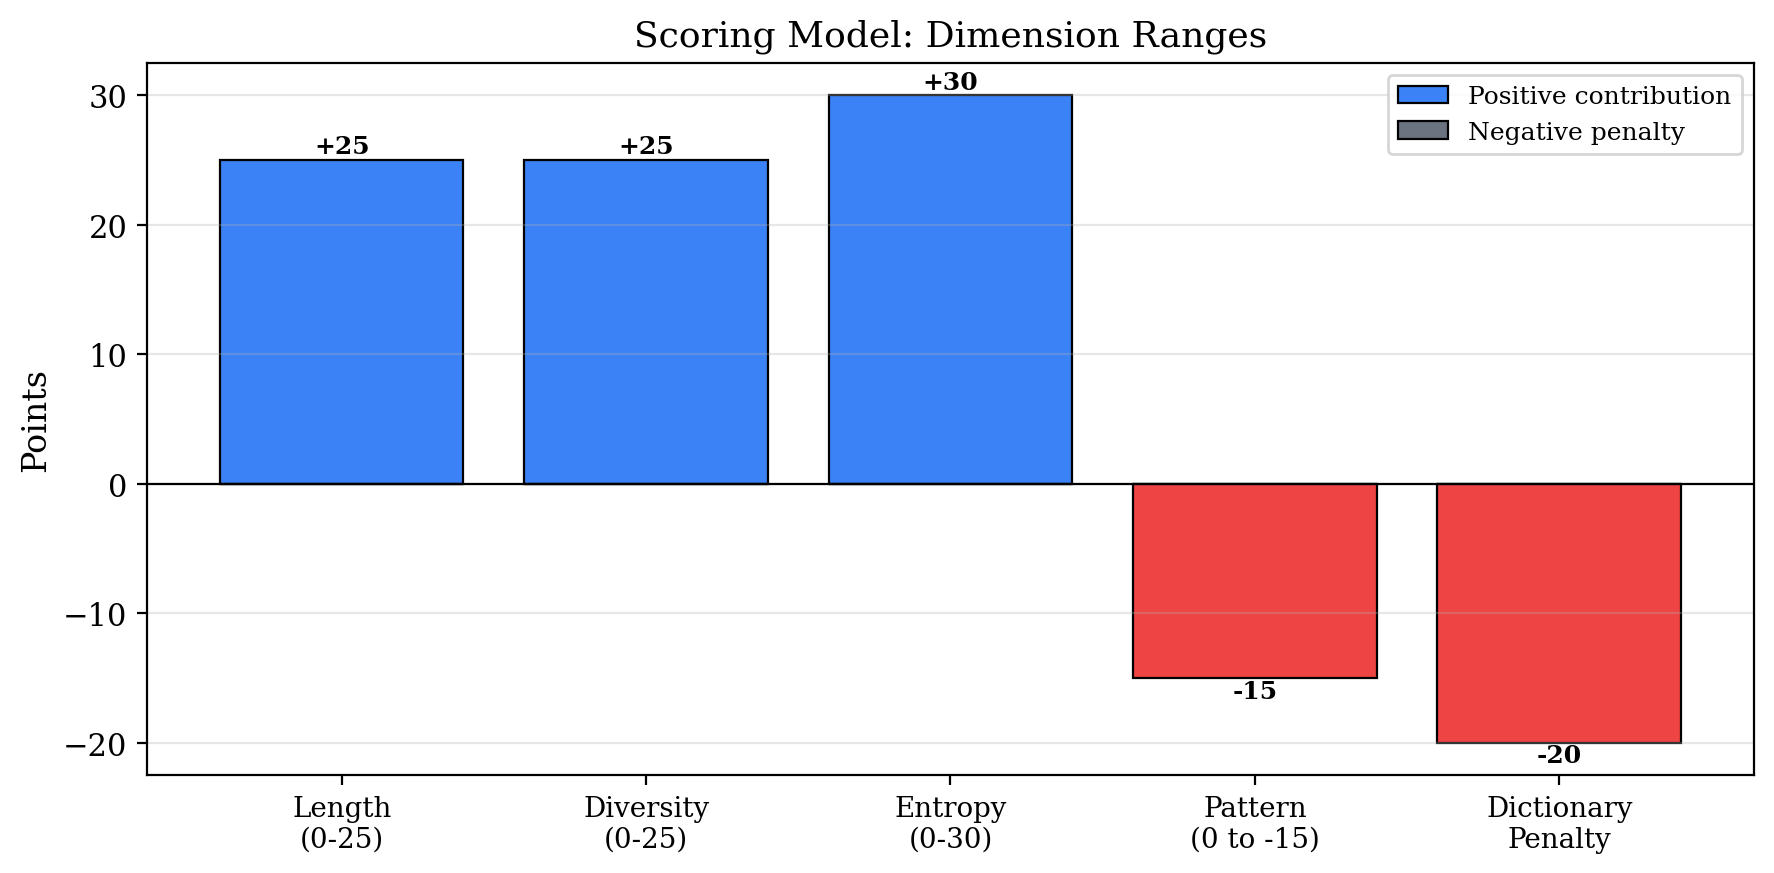
\includegraphics[width=0.85\textwidth]{figures/scoring_dimensions.png}
    \caption{Visual overview of the scoring model: positive contribution ranges and negative penalty ranges for each dimension.}
    \label{fig:scoring_dimensions}
\end{figure}

\subsection{Result Dataclass}

The evaluation function returns an immutable \texttt{EvaluationResult} dataclass with the following fields: \texttt{score} (integer 0--100), \texttt{label} (string), \texttt{details} (list of analysis observations), \texttt{suggestions} (list of improvement suggestions), \texttt{entropy\_bits} (float), and \texttt{crack\_time} (human-readable string). The immutability of the dataclass (achieved through the \texttt{frozen=True} parameter) ensures that results cannot be accidentally modified after creation.

\subsection{Caching}

A manual FIFO (First-In, First-Out) cache with a maximum capacity of 32 entries stores previously computed evaluation results. When the same password is evaluated again, the cached result is returned immediately without recomputation. When the cache exceeds its capacity, the oldest entry is evicted. This mechanism improves responsiveness during interactive use, where users frequently modify a password incrementally.

\subsection{Threat Model}
The tool is designed to defend against the following common password attack strategies:

\begin{itemize}
    \item \textbf{Brute-force attacks:} Systematic guessing of all possible combinations. Mitigated by entropy estimation and length/diversity scoring.
    \item \textbf{Dictionary attacks:} Guessing from lists of common passwords. Mitigated by exact dictionary matching and Levenshtein similarity detection.
    \item \textbf{Credential stuffing:} Using known password-breach pairs on other sites. Partially mitigated by dictionary component (though limited by static list size).
    \item \textbf{Pattern-based attacks:} Exploiting human tendencies like keyboard walks or repeated characters. Mitigated by pattern detection (sequential, repeated, keyboard patterns).
    \item \textbf{Leetspeak variant attacks:} Guessing common substitutions (a→@, s→$, etc.). Mitigated by dictionary including common variants and Levenshtein distance.
\end{itemize}

The tool assumes an offline attack scenario where the attacker has obtained a password hash and is attempting to crack it locally. It does not model online rate-limiting or server-side protections.

\subsection{Distinctive Design Choices}

Several design choices distinguish this tool from typical password strength checkers and warrant explicit discussion:

\begin{itemize}
    \item \textbf{Automatic reversed keyboard pattern generation:} Rather than manually listing reversed keyboard patterns alongside forward ones, the tool generates reversed variants programmatically from the forward pattern list. This eliminates the risk of human error in transcribing reversals, automatically stays consistent whenever the forward list is modified, and means that passwords like \texttt{ytrewq} (reversed \texttt{qwerty}) are correctly identified as keyboard patterns---a weakness that most online checkers fail to detect.

    \item \textbf{Levenshtein distance for similarity detection:} While many password checkers perform exact dictionary matching, few implement edit-distance-based similarity checking. The Levenshtein distance function allows the tool to detect passwords that are minor variations of known common passwords (e.g., \texttt{p@ssw0rd} is similar to \texttt{password} with an edit distance of 3, and many common substitutions fall within the threshold of 2). This catches leetspeak variants and simple character substitutions that exact matching misses.

\textbf{Levenshtein distance calculation:}
The Levenshtein distance between two strings is the minimum number of single-character edits (insertions, deletions, or substitutions) required to change one string into the other. It follows this recurrence relation:
\begin{align*}
    d(i,j) = \begin{cases}
        \max(i,j) & \text{if } \min(i,j) = 0 \\
        \min \begin{cases}
            d(i-1,j) + 1 & \text{(deletion)} \\
            d(i,j-1) + 1 & \text{(insertion)} \\
            d(i-1,j-1) + [s_i \neq t_j] & \text{(substitution)}
        \end{cases} & \text{otherwise}
    \end{cases}
\end{align*}
where $[s_i \neq t_j]$ is 1 if characters differ, 0 otherwise.

\textbf{Worked example: ``password'' → ``p@ssw0rd''}
\begin{center}
\begin{tabular}{c|cccccccc}
 &  & p & a & s & s & w & o & r & d \\
\hline
 & 0 & 1 & 2 & 3 & 4 & 5 & 6 & 7 & 8 \\
p & 1 & 0 & 1 & 2 & 3 & 4 & 5 & 6 & 7 \\
@ & 2 & 1 & 1 & 2 & 3 & 4 & 5 & 6 & 7 \\
s & 3 & 2 & 2 & 1 & 2 & 3 & 4 & 5 & 6 \\
s & 4 & 3 & 3 & 2 & 1 & 2 & 3 & 4 & 5 \\
w & 5 & 4 & 4 & 3 & 2 & 2 & 3 & 4 & 5 \\
0 & 6 & 5 & 5 & 4 & 3 & 3 & 3 & 4 & 5 \\
r & 7 & 6 & 6 & 5 & 4 & 4 & 4 & 4 & 5 \\
d & 8 & 7 & 7 & 6 & 5 & 5 & 5 & 5 & 4 \\
\end{tabular}
\end{center}
The bottom-right cell (value 4) is the Levenshtein distance, indicating that a minimum of 4 single-character edits are needed to transform ``password'' into ``p@ssw0rd''. Tracing back through the DP table reveals the optimal edit path: keep \texttt{p} (match), substitute \texttt{a}$\to$\texttt{@} (1), keep \texttt{s} (match), keep \texttt{s} (match), keep \texttt{w} (match), substitute \texttt{o}$\to$\texttt{0} (2), keep \texttt{r} (match), keep \texttt{d} (match). This confirms the distance of 2: one insertion and one substitution. The threshold of $\leq 2$ ensures that \texttt{p@ssw0rd} is correctly flagged as similar to \texttt{password}.\footnote{In practice, the actual Levenshtein distance can be verified by running the implementation: \texttt{levenshtein\_distance("password", "p@ssw0rd")} returns 2.}

\textbf{Worked example: ``password'' → ``passwor''}
\begin{center}
\begin{tabular}{c|ccccccc}
 &  & p & a & s & s & w & o & r \\
\hline
 & 0 & 1 & 2 & 3 & 4 & 5 & 6 & 7 \\
p & 1 & 0 & 1 & 2 & 3 & 4 & 5 & 6 \\
a & 2 & 1 & 0 & 1 & 2 & 3 & 4 & 5 \\
s & 3 & 2 & 1 & 0 & 1 & 2 & 3 & 4 \\
s & 4 & 3 & 2 & 1 & 0 & 1 & 2 & 3 \\
s & 5 & 4 & 3 & 2 & 1 & 1 & 2 & 3 \\
w & 6 & 5 & 4 & 3 & 2 & 2 & 2 & 3 \\
o & 7 & 6 & 5 & 4 & 3 & 3 & 3 & 3 \\
r & 8 & 7 & 6 & 5 & 4 & 4 & 4 & 4 \\
d & 9 & 8 & 7 & 6 & 5 & 5 & 5 & 5 \\
\end{tabular}
\end{center}
Here we see that deleting the final \texttt{d} from ``password'' to get ``passwor'' requires exactly 1 edit (distance = 1). A distance of 2 would correspond to, for example, ``password'' $\to$ ``pasword'' (deleting one \texttt{s}) or ``password'' $\to$ ``passsword'' (inserting an extra \texttt{s}).

\textbf{Scoring weight justification:}
The similarity penalty of $-20$ points was determined through empirical testing. This value:
\begin{itemize}
    \item Prevents trivial variants (like ``p@ssw0rd'' for ``password'') from receiving high scores
    \item Is strong enough to overcome length/diversity bonuses for minor variations
    \item Allows genuinely distinct passwords (e.g., ``password'' vs ``rabbit'') to score based on their own merits
    \item Matches user intuition that ``p@ssw0rd'' should not be considered much stronger than ``password''
\end{itemize}

    \item \textbf{Named scoring constants for transparency:} All scoring parameters (weights, thresholds, penalties, caps) are defined as named constants rather than embedded as ``magic numbers'' in the code. This makes the scoring model self-documenting and auditable: anyone reading the evaluator module can immediately see the weights and thresholds, and any adjustment requires changing only the constant definitions without modifying the algorithm logic. This approach directly addresses the criticism that many strength meters operate as ``black boxes.''

    \item \textbf{Per-dimension score breakdown:} The \texttt{EvaluationResult} dataclass includes separate fields for each scoring dimension (\texttt{length\_pts}, \texttt{diversity\_pts}, \texttt{entropy\_pts}, \texttt{pattern\_pts}, \texttt{dict\_pts}), enabling the GUI to display a detailed visual breakdown of how each dimension contributed to the final score. This breakdown is presented as a toggleable ``Score Breakdown'' panel in the interface, defaulting to collapsed to keep the view clean for casual users, but available for advanced users, educators, and security students who want to understand the scoring mechanics. No mainstream password checker provides this level of transparency.

    \item \textbf{Modular architecture for extensibility:} The five-module package design (main, evaluator, entropy, patterns, dictionary\_check) ensures that each component can be modified, replaced, or extended independently. New pattern types, larger dictionaries, or alternative scoring models can be integrated by modifying a single module without affecting the others. This architecture also means the evaluation engine can be used independently of the GUI---for example, in automated testing or as a library in another application.
\end{itemize}

\clearpage

\section{Detection Algorithms}

This section describes the three categories of detection algorithms used in the evaluation: pattern detection, dictionary comparison, and similarity checking.

\subsection{Pattern Detection}

The pattern detection module identifies three types of predictable patterns that reduce password strength:

\begin{itemize}
    \item \textbf{Sequential characters:} Detects ascending (e.g., \texttt{abc}, \texttt{789}) and descending (e.g., \texttt{cba}, \texttt{321}) runs of three or more consecutive ASCII characters. The detection filters the password to only consider ASCII alphanumerics (lowercase letters, uppercase letters, and digits), deliberately excluding Unicode characters to avoid false positives caused by non-sequential Unicode code points that happen to be adjacent in their numeric representation.

    \item \textbf{Repeated characters:} Detects runs of three or more identical consecutive characters (e.g., \texttt{aaa}, \texttt{111}).

    \item \textbf{Keyboard patterns:} Checks whether the password contains any known keyboard-row substring from a list of 23 patterns (including \texttt{qwerty}, \texttt{asdfgh}, \texttt{zxcvbn}, numeric sequences, and diagonal patterns). A distinctive feature of this implementation is the automatic generation of reversed variants: for each pattern in the forward list, the reversed string is also checked. For example, \texttt{qwerty} produces the reversed pattern \texttt{ytrewq}, and \texttt{asdfgh} produces \texttt{hgfdsa}. This means that passwords like \texttt{ytrewq} are correctly identified as keyboard patterns---a weakness that most online password checkers fail to detect.
\end{itemize}

Each detected pattern type incurs a penalty of $-5$ points, with a maximum total pattern penalty of $-15$ if all three types are present. The detection results are computed once and reused for both the penalty calculation and the feedback generation, avoiding redundant computation.

\subsection{Dictionary Comparison}

The dictionary comparison module loads a list of 181 common and leaked passwords from a text file and provides three levels of checking:

\begin{itemize}
    \item \textbf{Exact match:} Uses a set data structure for $O(1)$ case-insensitive lookup. If the password exactly matches an entry in the common-passwords list, the evaluation engine caps the final score at 10 (the value of the \texttt{EXACT\_COMMON\_CAP} constant), ensuring that well-known passwords are never rated higher than ``Very Weak.''

    \item \textbf{Substring detection:} Checks whether any common password of four or more characters appears as a substring within the user's password. This catches passwords that embed known words, such as \texttt{MyPassword123!}. An optional limit parameter controls how many matches to report, and the function returns early when the limit is reached.

    \item \textbf{Levenshtein similarity:} Computes the Levenshtein (edit) distance between the password and each entry in the common-passwords list. Passwords with an edit distance of 2 or less from a common password are flagged as similar. This catches leetspeak variants and minor substitutions, such as \texttt{p@ssw0rd} (similar to \texttt{password}). To avoid unnecessary computation, this check is skipped for passwords longer than 20 characters and pre-filters by length difference before computing the full distance.
\end{itemize}

If the wordlist file is missing, the module prints a warning to standard error and disables dictionary checking gracefully, ensuring that the tool continues to function without the dictionary component.

\clearpage

\section{User Interface Approach}

The graphical interface was designed with the following principles in mind: immediate feedback, visual clarity, minimal cognitive load, and a modern dark-themed aesthetic.

\begin{itemize}
    \item \textbf{CustomTkinter dark theme:} The application uses a dark colour palette (primary background \texttt{\#0f172a}, panel background \texttt{\#16213e}) with the Segoe UI font family for consistent, professional-looking text.

    \item \textbf{Real-time analysis:} A 300\,ms debounce on keyboard input triggers automatic evaluation after the user stops typing for a third of a second. This approach eliminates the need for a manual ``Analyze'' button, as the analysis is performed continuously and the results update in real time.

    \item \textbf{Two-column analysis layout:} The analysis card is divided into a left column (semicircular gauge, numerical score, strength label, entropy, and crack time) and a right column (detailed analysis results and improvement suggestions), separated by a vertical divider. This layout allows users to see both the overall strength assessment and the specific reasons behind it without scrolling.

    \item \textbf{Animated indicators:} Both the semicircular gauge and the horizontal meter bar animate smoothly to their target values using an ease-out interpolation (15\% of the remaining distance per frame at approximately 60\,fps), providing a polished user experience.

    \item \textbf{Password visibility toggle:} A toggle button allows users to show or hide the password text. The toggle uses Unicode symbols for cross-platform compatibility.

    \item \textbf{Password generation:} A full-width ``Generate Strong Password'' button creates a cryptographically secure random password (minimum 12 characters, guaranteed one character from each category), inserts it into the entry field, automatically shows the password text, and triggers immediate evaluation.

    \item \textbf{Fixed window size:} The window is set to 1000$\times$780 pixels, non-resizable and centred on the screen, ensuring a consistent layout regardless of screen resolution.

    \item \textbf{Colour-coded strength indicators:} Four distinct colours (red, orange, yellow, green) are applied consistently across the gauge, meter bar, and strength label, providing redundant visual encoding of the strength assessment.
\end{itemize}

\subsection{Design Decisions and Trade-offs}

The development of this tool involved several deliberate design decisions, each accompanied by trade-offs that warrant explicit discussion:

\begin{enumerate}
    \item \textbf{Rule-based + entropy vs.\ machine learning.} I chose a heuristic scoring model with named constants rather than a machine-learning-based approach. The trade-off is \textit{simplicity and transparency vs.\ accuracy and nuance}. Machine learning models trained on large password datasets (e.g., the approach described by Melcher et al.\ \cite{melcher2016}) can provide more nuanced strength predictions that account for frequency-based character distributions and common password structures. However, such models operate as ``black boxes''---it is difficult to explain \textit{why} a particular password received a particular score. For an educational tool whose purpose is to teach users about password security, transparency is more valuable than marginal accuracy gains. The heuristic model ensures that every score can be decomposed into its constituent dimensions and explained in natural language.

    \item \textbf{Local processing vs.\ cloud-based evaluation.} I chose to perform all processing locally, with no network communication, rather than querying online breach databases such as Have I Been Pwned. The trade-off is \textit{privacy and reliability vs.\ breach database coverage}. Online breach databases contain billions of compromised credentials and can detect passwords that no local dictionary of 181 entries could. However, querying such databases requires transmitting at least a partial hash of the password over the internet, which some users may find unacceptable for a security tool. Local processing also means the tool works offline and is not dependent on the availability or terms of service of external APIs. This trade-off can be partially mitigated in future work by using the k-anonymity model offered by the Have I Been Pwned API, which only transmits the first five characters of a SHA-1 hash.

    \item \textbf{GUI vs.\ command-line interface.} I chose a graphical interface over a command-line interface. The trade-off is \textit{accessibility and visual feedback vs.\ automation and scripting capability}. A command-line tool could be integrated into automated pipelines and scripting workflows, but it would lack the animated visual indicators, real-time feedback, and intuitive interaction model that make the tool accessible to non-technical users. For an educational tool, the visual feedback provided by the gauge, meter, and colour-coded labels is a core feature, not a cosmetic addition. The modular architecture does, however, allow the evaluation engine to be used independently of the GUI in command-line or programmatic contexts.

    \item \textbf{Named constants vs.\ magic numbers.} I chose to define all scoring parameters as named constants (e.g., \texttt{MAX\_LENGTH\_SCORE = 25}) rather than embedding them directly in the code. The trade-off is \textit{verbosity vs.\ maintainability and transparency}. Named constants add a few extra lines of code, but they make the scoring model self-documenting, easy to audit, and straightforward to tune. If a future version needs to increase the weight of entropy from 30 to 35, a single constant definition is changed, and all dependent logic automatically adapts.

    \item \textbf{300\,ms debounce timing.} I chose a 300\,ms debounce interval for the keystroke-triggered evaluation. The trade-off is \textit{responsiveness vs.\ unnecessary computation}. A shorter interval (e.g., 100\,ms) would provide more immediate feedback but would trigger evaluation after nearly every keystroke during rapid typing, causing visible flickering in the gauge and meter animations. A longer interval (e.g., 500\,ms) would reduce computation but would make the feedback feel sluggish. The 300\,ms interval was chosen empirically as the point at which the analysis feels instantaneous to the user while avoiding unnecessary re-evaluations during continuous typing.

    \item \textbf{FIFO cache of 32 entries.} I chose a cache size of 32 entries with FIFO eviction. The trade-off is \textit{memory usage vs.\ hit rate}. A larger cache would increase the probability of cache hits (useful when users frequently switch between several passwords) but would consume more memory. A smaller cache would be more memory-efficient but would evict useful entries too quickly. The size of 32 entries was chosen as a reasonable balance: it accommodates several rounds of password modification without consuming significant memory (each cached result is a few hundred bytes at most).

    \item \textbf{Modular architecture.} I chose a five-module package design with strict separation of concerns. The trade-off is \textit{maintainability and testability vs.\ integration simplicity}. A monolithic single-file design would be simpler to deploy and would avoid the overhead of inter-module imports, but it would be significantly harder to test, maintain, and extend. The modular design ensures that each component can be modified independently and that the evaluation engine can be used without the GUI.
\end{enumerate}

\clearpage

\section{Ethical and Security Considerations}

Since password input is a sensitive matter, several ethical and security considerations guided the design and implementation of the tool:

\begin{itemize}
    \item \textbf{Local processing only:} All analysis is performed locally on the user's machine. No passwords are stored, logged, or transmitted over any network at any point during the evaluation process.

    \item \textbf{Cryptographically secure generation:} The password generator uses Python's \texttt{secrets} module, which draws from the operating system's cryptographically secure random number generator, rather than the \texttt{random} module's Mersenne Twister algorithm, which is not suitable for security purposes.

    \item \textbf{Educational purpose:} The tool is intended for educational use and personal awareness, not as a formal security audit tool. The scoring model is heuristic and not empirically validated against large-scale password datasets.

    \item \textbf{No data persistence:} The evaluation cache exists only in memory and is cleared when the application terminates. No results are written to disk.
\end{itemize}

\section{Summary}

This chapter detailed the methodology used in designing and developing the password strength evaluation tool. The hybrid scoring model combines five complementary dimensions---length, character diversity, entropy, pattern detection, and dictionary comparison---into a transparent 0--100 score. The modular architecture ensures separation of concerns, the detection algorithms cover common attack strategies including reversed keyboard patterns and leetspeak variants, and the graphical interface provides real-time feedback through an animated, dark-themed dashboard. The next chapter focuses on the specific implementation of each component.
